\section{Design choices}
In this section we will present the design choices. First, notice that the stream cipher module shall be reset before its usage. Whenever the reset signal is asserted, other signals are ignored. Reset is negedge triggered.

Secondly, all the logic of the stream cipher module (except the S-box) is synchronous.

\subsection{S-box}
We have implemented the S-box in a separate module with respect to the stream cipher for higher reusability and to respect the Single Responsibility Principle.

In particular, we have implemented it as a lookup-table in continuous assignment. The S-box is defined as a packed two-dimensions array:
\begin{lstlisting}
wire [0:255][7:0] sbox;
\end{lstlisting}
S-box elements have been assigned in continuous assignments as following:
\begin{lstlisting}
assign sbox[8'h00] = 8'h63;
assign sbox[8'h01] = 8'h7c;
/* other 254 assignments... */
\end{lstlisting}
The module takes an input of 8-bits and outputs the result of the lookup as an 8-bit value. This is done in a continuous assignment too:
\begin{lstlisting}
assign out = sbox[in];
\end{lstlisting}

\subsection{Key management}

To keep the key correctly stored inside the module, we use an internal counter block (\lstinline{cb}), which is defined as an 8-bit \lstinline{reg}.

On reset, the counter block is set to zero as a default value. An additional 1-bit input signal (\lstinline{key_in}) has been added to allow to set the key. To correctly set the key, the \lstinline{key} signal must contain the key and must be stable, and the \lstinline{key_in} signal must be asserted. When these conditions are met, the key will be saved into the internal counter block \lstinline{cb} at the next rising edge of the clock. Moreover, there will be no output the next clock cycle, therefore we also deassert the \lstinline{dout_valid} signal.

\subsection{Other signals handling}
When the 1-bit \lstinline{din_valid} signal is asserted, the 8-bit input signal \lstinline{din} must to be valid and stable. The \lstinline{din} signal value is XORed with the result of the lookup in the S-box of the counter block \lstinline{cb} and it is stored in \lstinline{dout}, and \lstinline{dout_valid} is asserted. If \lstinline{din_valid} is not asserted, \lstinline{dout_valid} is deasserted. The \lstinline{dout} signal shall not be considered when \lstinline{dout_valid} is deasserted, as per specification.

Every clock cycle, if \lstinline{din_valid} is asserted (and \lstinline{key_in} is not), the counter block is increased by one modulo $256$. Notice that the modulo addition is implemented as a simple sum on an 8-bit \lstinline{reg}, which implicitly overflows (without any warning or error generated from used tools). We decided to implement it this way because we found out that it performed better (about $5 MHz$ increase) with respect to other possible implementations.

\clearpage
\section{Block diagram}
The top-level view of our module is represented in \cref{fig:top_level}, with every input and output.

\lstset{basicstyle=\large\ttfamily}
\begin{figure}[!ht]
    \centering
    \begin{circuitikz}
        \tikzset{box/.style = {draw=black, thick,minimum height=5cm, text width=5cm,align=center}}
        \node (GCR) [box] {\parbox{4cm}{\Large\centering AES S-box based\\stream cipher}};

        \draw ($(GCR.south west)!1!(GCR.south)$) -- ++(0,-.5) node[anchor=north]{\lstinline{clk}};
        \draw ($(GCR.south west)!1!(GCR.south)$) ++(-.25,0.01) -- ++(0.25,0.25);
        \draw ($(GCR.south west)!1!(GCR.south)$) ++(.25,0.01) -- ++(-0.25,0.25);

        \draw [<-,>=stealth]($(GCR.north west)!.3!(GCR.west)$) -- ++(-1,0) node[anchor=east]{\lstinline{din}};
        \draw [<-,>=stealth]($(GCR.north west)!.6!(GCR.west)$) -- ++(-1,0) node[anchor=east]{\lstinline{din_valid}};
        \draw [<-,>=stealth]($(GCR.north west)!.9!(GCR.west)$) -- ++(-1,0) node[anchor=east]{\lstinline{key}};
        \draw [<-,>=stealth]($(GCR.north west)!1.2!(GCR.west)$) -- ++(-1,0) node[anchor=east]{\lstinline{key_in}};
        \draw [<-,>=stealth]($(GCR.north west)!1.7!(GCR.west)$) -- ++(-1,0) node[anchor=east]{\lstinline{rst_n}};

        \draw [->,>=stealth]($(GCR.north east)!0.75!(GCR.east)$) -- ++(1,0) node[anchor=west] {\lstinline{dout}};
        \draw [->,>=stealth]($(GCR.north east)!1.25!(GCR.east)$) -- ++(1,0) node[anchor=west] {\lstinline{dout_valid}};
    \end{circuitikz}
    \caption{Top-level view of the AES S-box based stream cipher}
    \label{fig:top_level}
\end{figure}
\lstset{basicstyle=\small\ttfamily}

We are now going to describe the synthesized netlist in all of its parts. For the full picture, please refer to the next page.

The update of the counter block \lstinline{cb} is implemented with a simple adder, where the result is used only when \lstinline{din_valid} is asserted. However, if \lstinline{key_in} is asserted, the update for the counter block register \lstinline{cb} is taken from the \lstinline{key} signal instead.
\begin{figure}[!ht]
    \centering
    \includegraphics[width=1\textwidth]{key_manage_netlist}
    \caption{Key management}
    \label{fig:key_manage_netlist}
\end{figure}

\clearpage
\newgeometry{top=0pt, bottom=0pt, left=0pt, right=0pt}
\begin{figure}
    \thispagestyle{empty}
    \centering
    \hspace*{-9cm}
    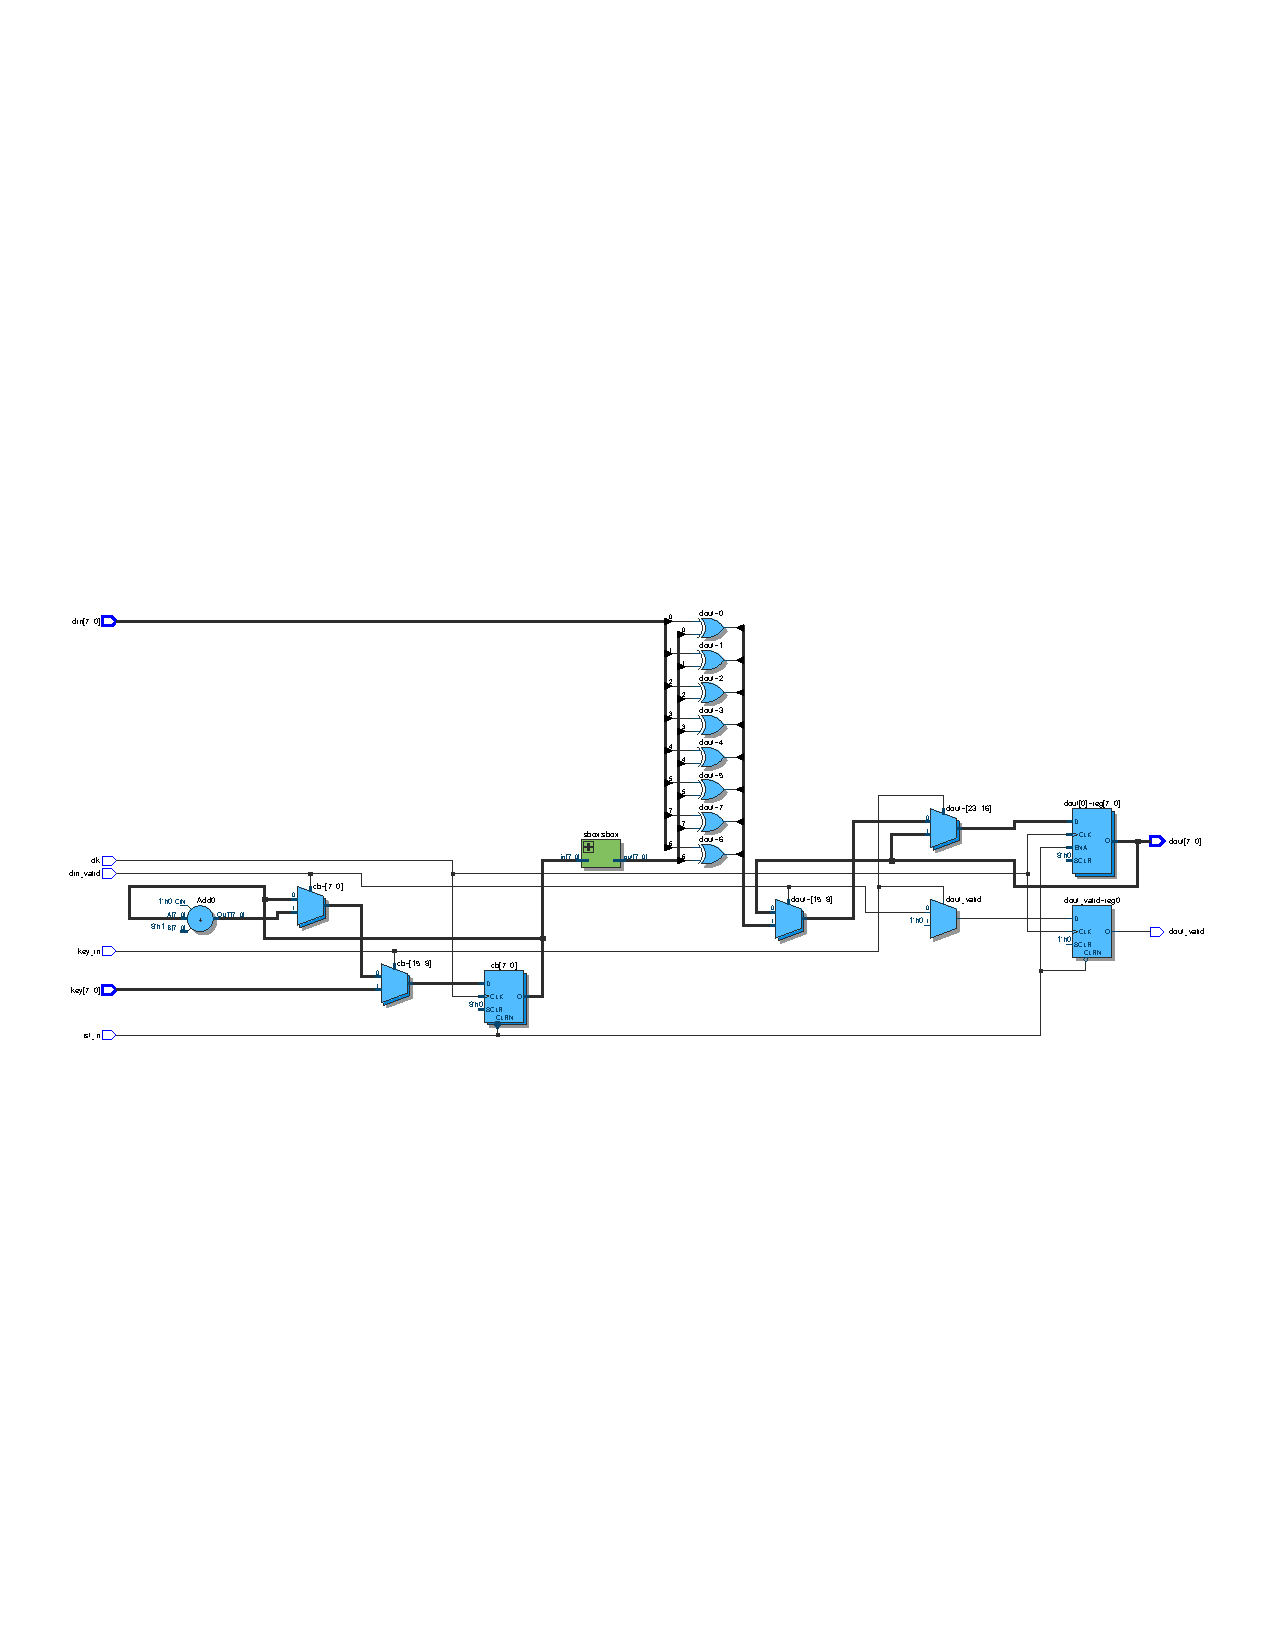
\includegraphics[width=1\textheight, angle=90]{complete_netlist}
\end{figure}
\restoregeometry
\clearpage

The S-box (\cref{fig:sbox_netlist}) is implement with 8 multiplexer in parallel with an 8-bit selection signal.
\begin{figure}[!ht]
    \centering
    \includegraphics[width=1\textwidth]{sbox_netlist}
    \caption{S-box netlist}
    \label{fig:sbox_netlist}
\end{figure}

The encryption (\cref{fig:encryption_netlist}) is a simple XOR cascade where the two inputs are the \lstinline{din} signal and the output of the S-box lookup of the counter block \lstinline{cb}.
\begin{figure}
    \centering
    \includegraphics[width=.5\textwidth]{encryption_netlist}
    \caption{Encryption netlist}
    \label{fig:encryption_netlist}
\end{figure}

Finally, we have the output handling (\cref{fig:output_netlist}). The \lstinline{key_in} signal and the \lstinline{din_valid} signal control whether to update \lstinline{dout} with a new value or to keep the old one. This is done by selecting the multiplexers input line. When the \lstinline{key_in} signal is asserted, the \lstinline{dout_valid} signal gets deasserted.
\begin{figure}
    \centering
    \includegraphics[width=1\textwidth]{output_netlist}
    \caption{Output netlist}
    \label{fig:output_netlist}
\end{figure}